\documentclass{beamer}

%% Use package -----------------------------------------------------------------

\usepackage[T1]{fontenc}
\usepackage[utf8]{inputenc}
\usepackage{lmodern}
\usepackage{graphicx}
\usepackage[absolute,overlay]{textpos}
\usepackage{multicol}
\usepackage{listings}

\usepackage{multimedia}

\usepackage{svg}




%% Beamer customization---------------------------------------------------------

\usepackage{xcolor}
\usetheme{Warsaw}

%% Themes
% Outer themes
\useoutertheme{shadow}
% Rounded boxes and shadows
\useinnertheme[shadow=true]{rounded}
% Solid \item symbols
\useinnertheme{circles}

%% Custom colors
\definecolor{rltgreen}{rgb}{0,0.5,0}
\definecolor{pasteur}{RGB}{0,90,154}
\setbeamerfont{block title}{size={}}
\setbeamercolor{structure}{fg=pasteur}
\setbeamercolor{item}{fg=pasteur}

%Color of title
\setbeamertemplate{frametitle}
{
    \nointerlineskip
    \begin{beamercolorbox}[sep=0.3cm,ht=1.8em,wd=\paperwidth]{frametitle}
        \vbox{}\vskip-2ex%
        \strut\insertframetitle\strut
        \vskip-0.8ex%
    \end{beamercolorbox}
}
% Hide navigation symbols
\setbeamertemplate{navigation symbols}{}

%% Title block
\setbeamercolor*{title}{use=structure,fg=white,bg=pasteur}

%% Bottom infolines
\setbeamertemplate{footline}
{
  \leavevmode%
  \hbox{%
  \begin{beamercolorbox}[wd=.3\paperwidth,ht=2.25ex,dp=1ex,center]{author in head/foot}%
    \usebeamerfont{author in head/foot}\insertshortauthor
  \end{beamercolorbox}%
  \begin{beamercolorbox}[wd=.7\paperwidth,ht=2.25ex,dp=1ex,center]{title in head/foot}%
    \usebeamerfont{title in head/foot}\insertshorttitle\hspace*{3em}
    \insertframenumber{} / \inserttotalframenumber\hspace*{1ex}
  \end{beamercolorbox}}%
  \vskip0pt%
}
\makeatletter

%% Top infolines
\setbeamertemplate{headline}{%
\leavevmode%
  \hbox{%
    \begin{beamercolorbox}[wd=\paperwidth,ht=2.5ex,dp=1.125ex]{palette quaternary}%
    \insertsectionnavigationhorizontal{\paperwidth}{}{\hskip0pt plus1filll}
    \end{beamercolorbox}%
  }
}

%% Define Snakemake ------------------------------------------------------------

\definecolor{eclipseBlue}{RGB}{42,0.0,255}
\definecolor{eclipseGreen}{RGB}{63,127,95}
\definecolor{eclipsePurple}{RGB}{127,0,85}

\lstset{language=Python}
\lstset{
    basicstyle=\tiny\ttfamily,
    morekeywords={rule, output, shell, params, run, configfile, temp, threads, log},
    showstringspaces=false,
    commentstyle=\color{eclipseGreen}, % style of comments
    keywordstyle=\color{eclipsePurple}, % style of keywords
    stringstyle=\color{eclipseBlue}, % style of strings
}


%% Set up title ----------------------------------------------------------------

\title{Snakemake overview}
\author[T.Cokelaer]{Thomas Cokelaer}
\institute{Institut Pasteur}
\date{Dec. 12th 2016\\ Journée Snakemake}

\begin{document}

%% Title slide -----------------------------------------------------------------

\begin{frame}[plain]
    \titlepage
    \begin{textblock*}{5cm}(4.5cm,0.3cm)
        
\includegraphics[scale=0.09]{images/Institut_Pasteur.png}
    \end{textblock*}
\end{frame}


\section{Introduction}

\begin{frame}[plain]
  \begin{figure}
      \centering
      \includegraphics[scale=0.2]{images/equation.png}
  \end{figure}
\end{frame}


\begin{frame}
\frametitle{Think Makefile, think DAG}
    
   \centering \textbf{Snakemake is a workflow manager}\\
      
        \only<1> 
        {
            \begin{figure}
                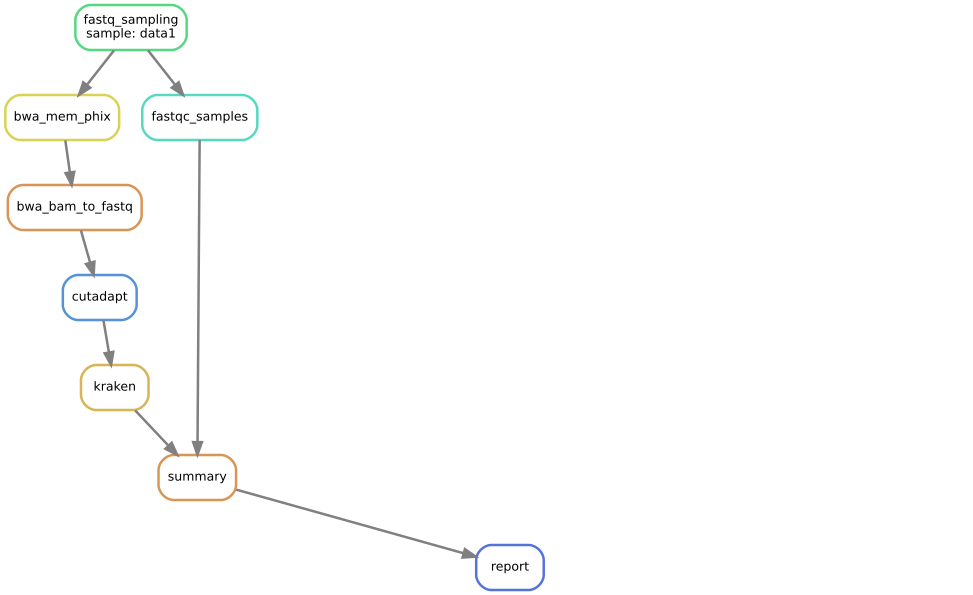
\includegraphics[width=\textwidth,height=0.6\textheight]{dag_0.png}
                \caption[1]{}
            \end{figure}                
        }
        \only<2> 
        {
            \begin{figure}
                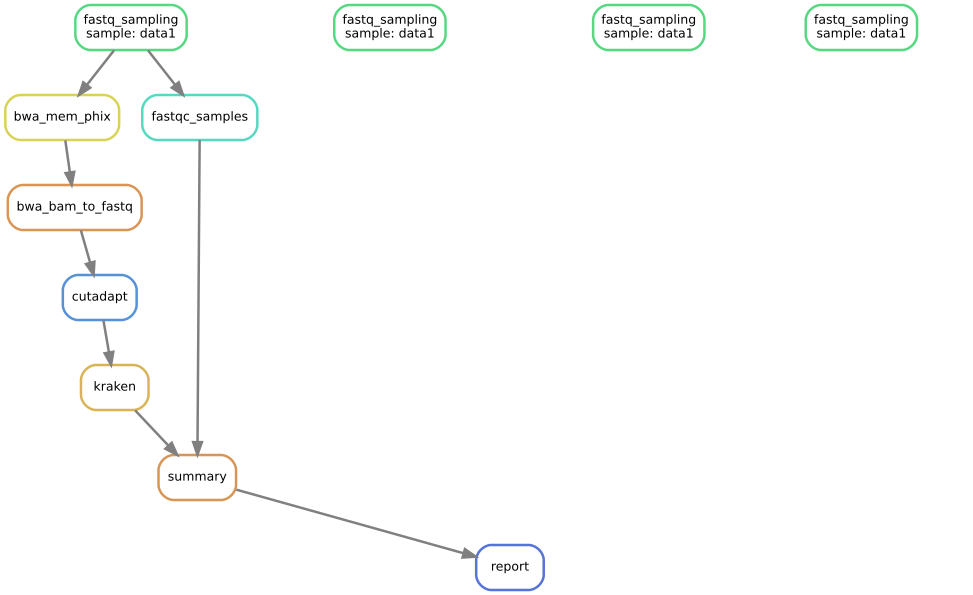
\includegraphics[width=\textwidth,height=0.6\textheight]{dag_1.png}
                \caption[1]{Ideal for embarassingly parallel problem}
            \end{figure}                
        }\only<3> 
        {
            \begin{figure}
                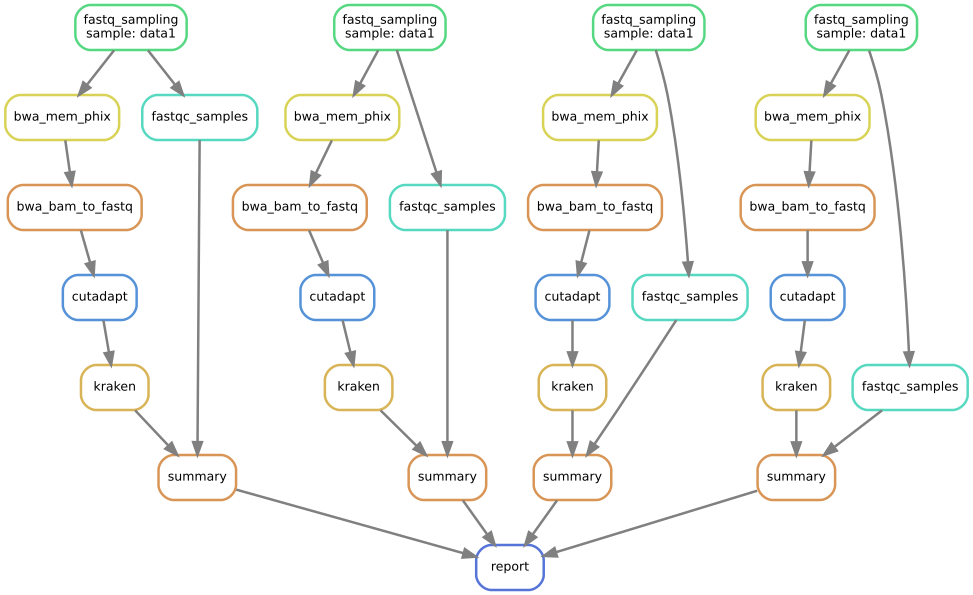
\includegraphics[width=\textwidth,height=0.6\textheight]{dag_2.png}
                \caption[1]{Ideal for embarassingly parallel problem}
            \end{figure}                
        }
        \only<4> 
        {
            \begin{figure}
                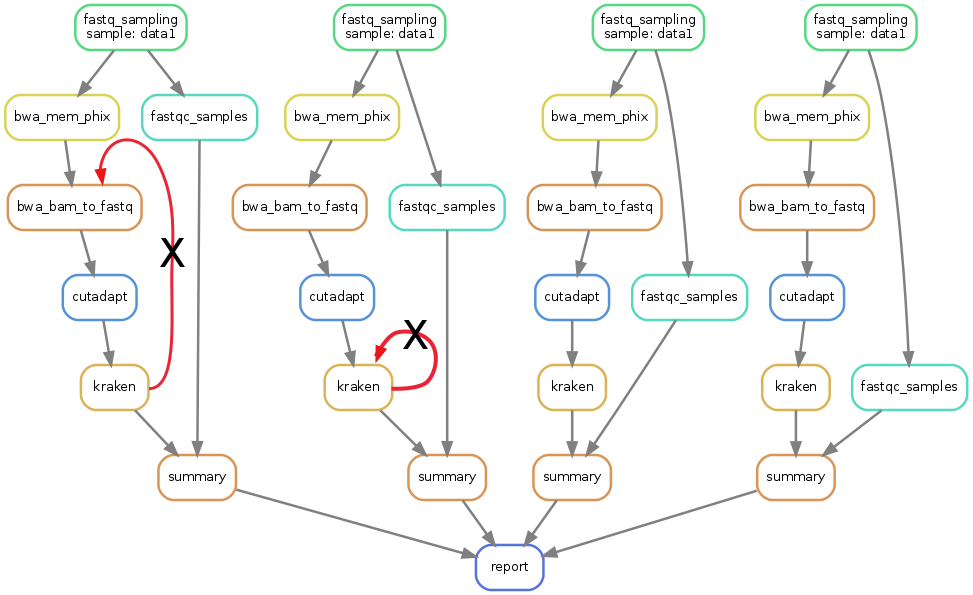
\includegraphics[width=\textwidth,height=0.6\textheight]{dag_wrong2.png}
                \caption[2]{Requires a DAG (no self loop of feedback loop allowed !)}
            \end{figure}
        }
  % Snakemake c'est plus que M + P
  % C'est aussi un workflow manager qui est PRATIQUE. 
  %Par forcement facile mais PRATIQUE.
\end{frame}


\begin{frame}
\frametitle{Growing community}
 \begin{figure}
 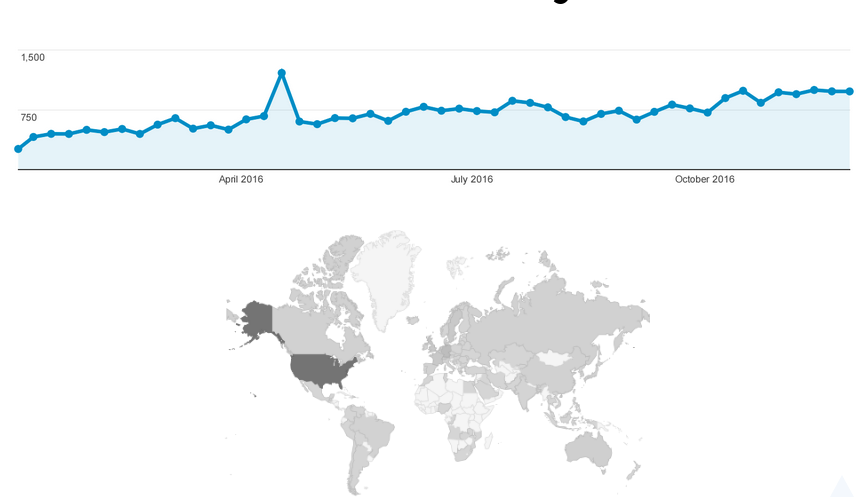
\includegraphics[scale=0.2]{images/community}
 \pause
 
\includegraphics[scale=0.2]{images/citations}
 \caption{References: slides.com/johanneskoester/snakemake-tutorial-2016}
 \end{figure}
\end{frame}



\begin{frame}
 \frametitle{Why is it successful}
 \centering
 \textbf{Python is a batteries included language. }

 \vspace{1cm}
 \pause
 \textbf{Snakemake as well !!}
 
 \pause
   \begin{itemize}
    \item  Clusters can be used with minimum efforts (no intrusive code)
    \item  Workflows can be run from or up to a given rule
    \item  Data provenance
    \item  Nice logging system to follows the status
    \item  Suspend /  Resume 
    \item  Various code can be integrated: R, bash, and of course Python
   \end{itemize}   
 
\end{frame}




%% Slides ----------------------------------------------------------------------

\section{Toy example}

\begin{frame}[plain]
 \centering
 \begin{Huge}
 From sequential commands to dependent rules: a toy example
 \end{Huge}
\end{frame}

% ------------------------------------------------------


\begin{frame}
\frametitle{The problem}
Let us consider two FastQ files (independent samples) and let us map them on a reference (phiX174). The two 
sample files are named sample\_A.fastq.gz and sample\_B.fastq.gz
  \begin{figure}
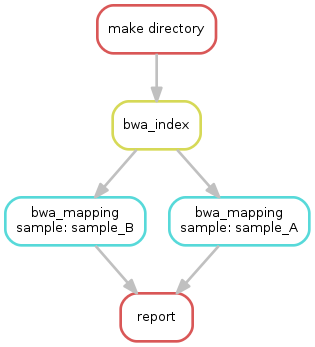
\includegraphics[width=0.5\textwidth, height=0.5\textheight]{tutorial/dag.png}
  \end{figure}
\end{frame}

% ------------------------------------------------------
 
 \begin{frame}[fragile, squeeze]
  \frametitle{The minimalist solution}

 \begin{columns}
 \begin{column}[T]{3cm}
 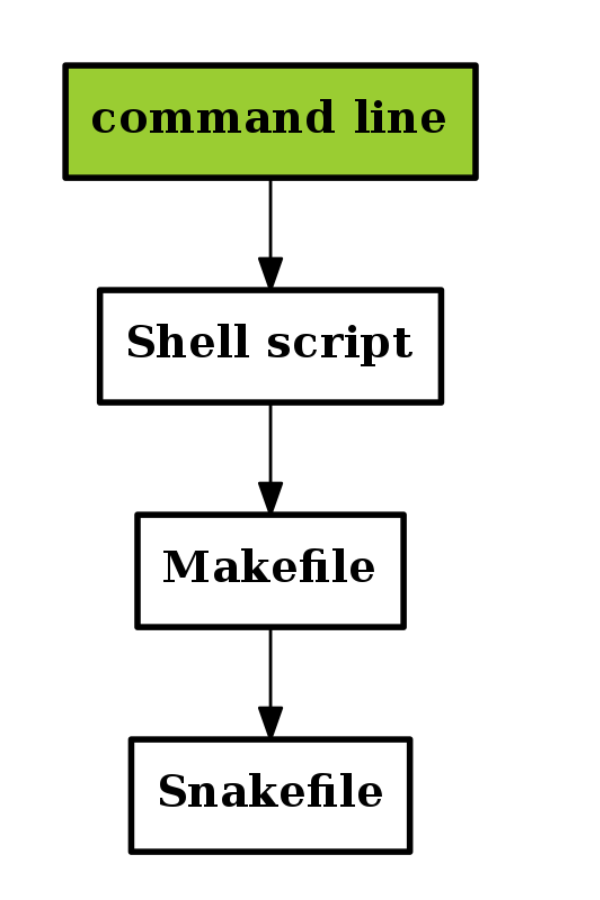
\includegraphics[width=1\textwidth, height=0.6\textheight]{images/flow_methods_1.png}
 \end{column}
  \begin{column}[T]{9cm}
  \begin{block}{Shell commands: pretty simple}
  \begin{lstlisting}
  # Create a directory
  mkdir -p mapped_sample
  
  # Build the index of the reference
  bwa index phiX174.fa
  
  # Do the mapping twice on the two input FastQ files
  bwa mem phiX174.fa A.fastq.gz | samtools view -Sb - > A.bam
  bwa mem phiX174.fa B.fastq.gz | samtools view -Sb - > B.bam
  \end{lstlisting}                                                      
  \end{block}
 \end{column}
 \end{columns}
 
 \pause
  \begin{alertblock}{Issues}
  Good start. Simple but what about some variables and scalability ?
  \end{alertblock}
 
\end{frame}


% ------------------------------------------------------

 \begin{frame}[fragile]
  \frametitle{A shell solution}  
 
 \begin{columns}
 \begin{column}[T]{3cm}
 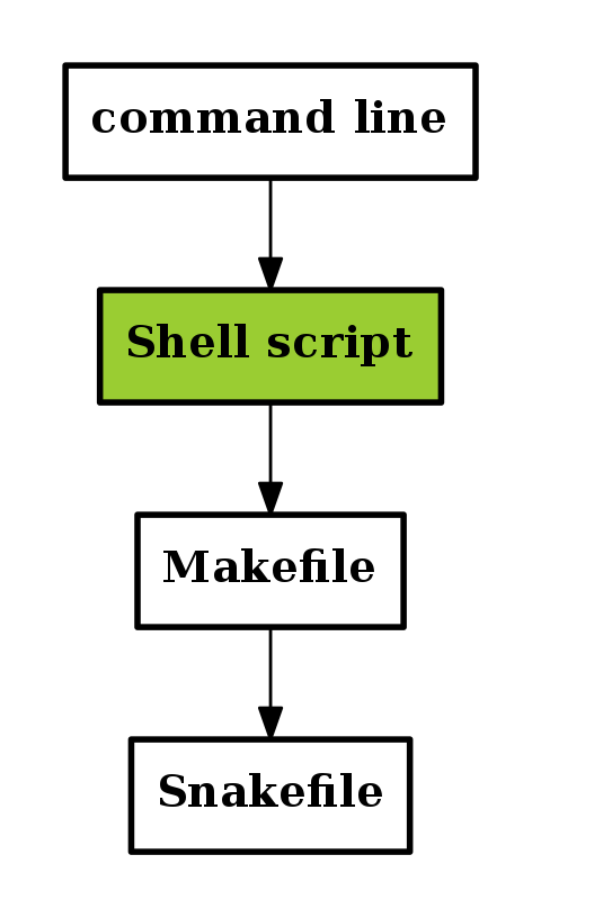
\includegraphics[width=1\textwidth, height=0.6\textheight]{images/flow_methods_2.png}
 \end{column}
  \begin{column}[T]{9cm}
 \begin{block}{Shell loop and variables}
  \begin{lstlisting}
#!/bin/sh
REFERENCE="phiX174.fa"
ODIR="mapped_sample"
SAMPLES=`ls *.fastq.gz` 

#Create a directory
mkdir -p $ODIR

# Build the index of the reference
bwa index $REFERENCE

# Do the mapping twice on the two input FastQ files
for var in $SAMPLES
do
   TARGET=${var/.fastq.gz/.bam}
   bwa mem $REFERENCE $SAMPLES | samtools view -Sb - > $ODIR/$TARGET
done
  \end{lstlisting}                                                      
  \end{block}
 \end{column}
\end{columns}
 
 
 \pause
  \begin{alertblock}{Issues}
  Still simple but sequential. What about dependencies between tasks ? What if a file exists already ? Do we start from scratch ?
  \end{alertblock} 
\end{frame}

% ------------------------------------------------------------


\begin{frame}[fragile]
  \frametitle{The Makefile solution: a set of directives (rules)}

   \begin{columns}
 \begin{column}[T]{3cm}
 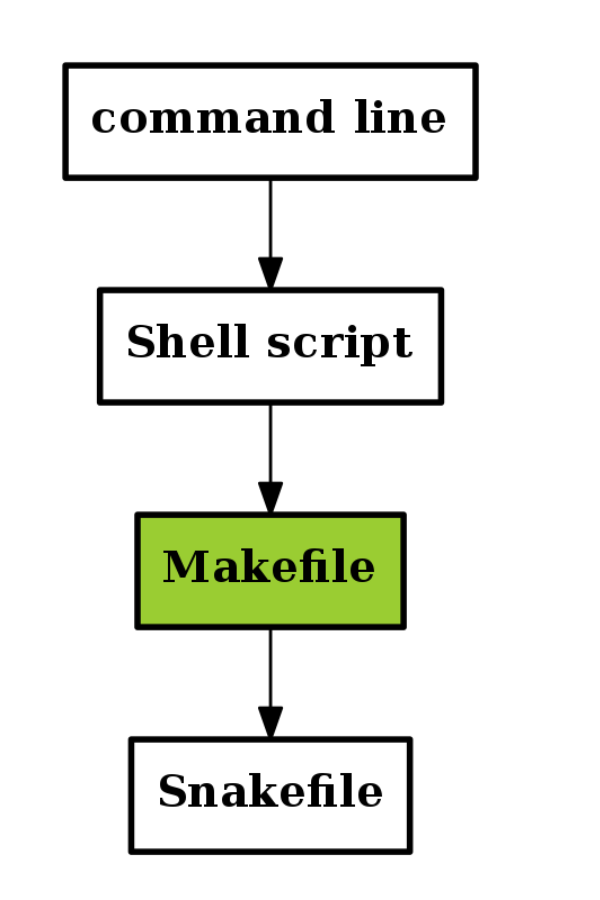
\includegraphics[width=1\textwidth, height=0.6\textheight]{images/flow_methods_3.png}
 \end{column}
  \begin{column}[T]{9cm}  
  A Makefile consists of a set of rules in the following form 
  \begin{block}{rule syntax}
  \begin{lstlisting}
target: dependencies
   system command(s)
   \end{lstlisting}
   \end{block}
   Makefile interests:\\
     - handles the dependencies between rules\\
     - avoids re-rerunning a task if the targets exist already\\   
   Widely used in C / C++ community for compilation of libraries. 
   \end{column}
   \end{columns}   
\end{frame}

% --------------------------------------------------

\begin{frame}[fragile]
    \frametitle{The Makefile solution: a set of directives (rules)}
    
    \begin{columns}
 \begin{column}[T]{3cm}
 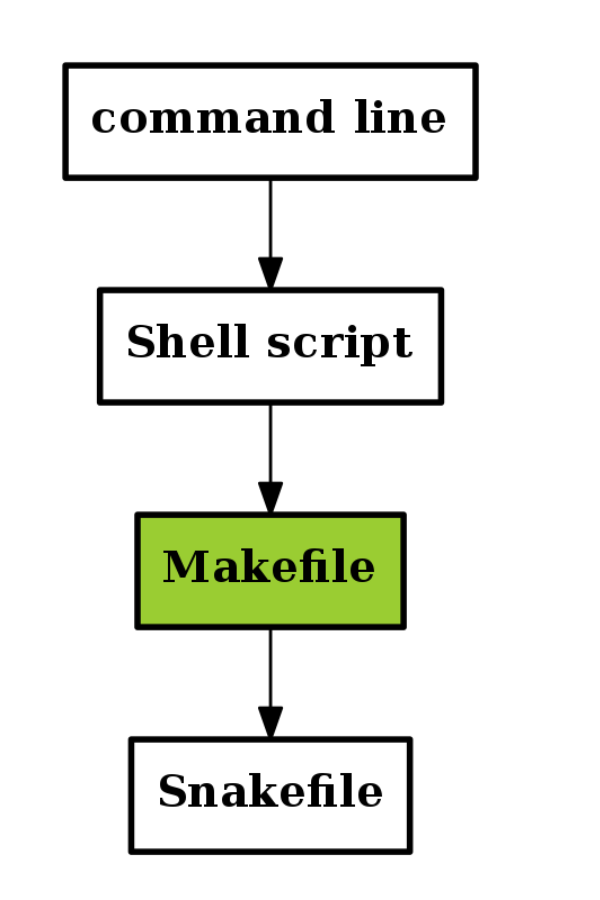
\includegraphics[width=1\textwidth, height=0.6\textheight]{images/flow_methods_3.png}
 \end{column}
  \begin{column}[T]{9cm}  
  
    \begin{block}{Makefile: a bwa\_mapping and bwa\_index rule}
    \small
    \begin{lstlisting}
SAMPLES = sample_A sample_B
ODIR = "mapped_sample"
FASTQS = $(patsubst %,%.fastq.gz,$(SAMPLES))
BAMS = $(patsubst %,$(ODIR)/%.bam,$(SAMPLES))

INDEX =  phiX174.fa.bwt
REFERENCE =  phiX174.fa

# Main rule
all: $(BAMS)

# bwa_mapping
$(ODIR)/%.bam: %.fastq.gz $(INDEX) $(ODIR)
  bwa mem $(REFERENCE) $< | samtools view -Sb - > $@

$(ODIR):
  mkdir -p $(ODIR)

# bwa_index
$(INDEX): $(REFERENCE)
  bwa index $<
    \end{lstlisting}
    \end{block}
  \end{column}
  \end{columns}
\end{frame}

% --------------------------------------------------------------------------

\begin{frame}[fragile]
    \frametitle{The Snakefile solution}
    
    \begin{columns}
 \begin{column}[T]{3cm}
 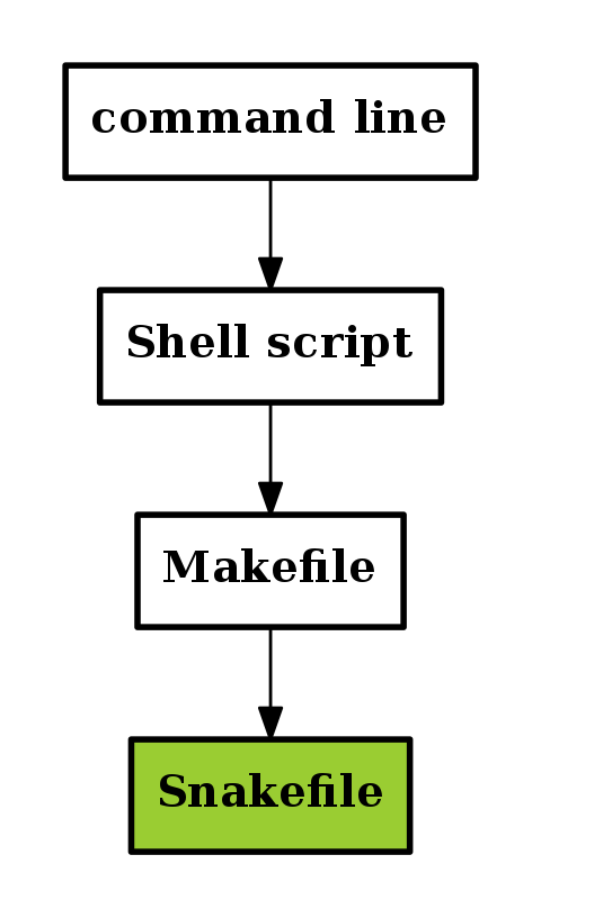
\includegraphics[width=1\textwidth, height=0.6\textheight]{images/flow_methods_4.png}
 \end{column}
  \begin{column}[T]{9cm}  
    \begin{block}{Snakefile}
    \begin{lstlisting}
SAMPLES = ["sample_A", "sample_B"]

rule all:
    input: expand("mapped_sample/{sample}.bam", sample=SAMPLES)

rule bwa_index:
    input: "phiX174.fa"
    output: "phiX174.fa.bwt"
    shell: "bwa index {input}"

rule bwa_mapping:
    input:
        ref = "phiX174.fa",
        index = "phiX174.fa.bwt",
        fastq = "{sample}.fastq.gz"
    output: "mapped_sample/{sample}.bam"
    shell:
        "bwa mem {input.ref} {input.fastq} | samtools view -Sb - > {output}"
    \end{lstlisting}
    \end{block}
    \end{column}
    \end{columns}
\end{frame}

\begin{frame}
 \frametitle{The Snakefile solution}
 \begin{block}{Snakemake logic: Makefile }
  Snakemake takes the best of Makefile: 
  \begin{itemize}
      \item infers dependencies and execution order
      \item rules define obtain output files from input files
      \item structured pipelines
  \end{itemize}
  \end{block}
  \begin{block}{Snakemake syntax: Python}
  \begin{itemize}
  \item Own domain specific syntax (rules and keywords)
  \item Use Python as the glue language
  \item The snakemake library itself is in Python
  \end{itemize}
  \end{block} 
\end{frame}


\section{Snakemake tutorial}

\begin{frame}[plain]
 \centering
 \begin{Huge}
 Snakemake tutorial
 \end{Huge}
\end{frame}

% --------------------------------



\begin{frame}
\centering
The problem: 

\begin{itemize}
 \item convert a WAV signal into a frequency plot (spectrogram)
 \item Repeat for N input files
 \item Effect of the time window parameter W on the resolution
\end{itemize}
 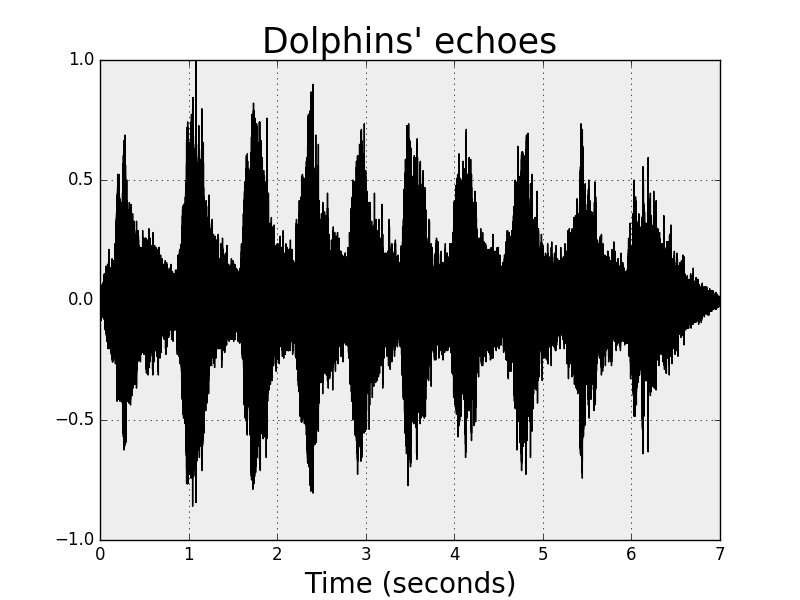
\includegraphics[scale=0.28]{images/dolphin_timeseries.png} 
 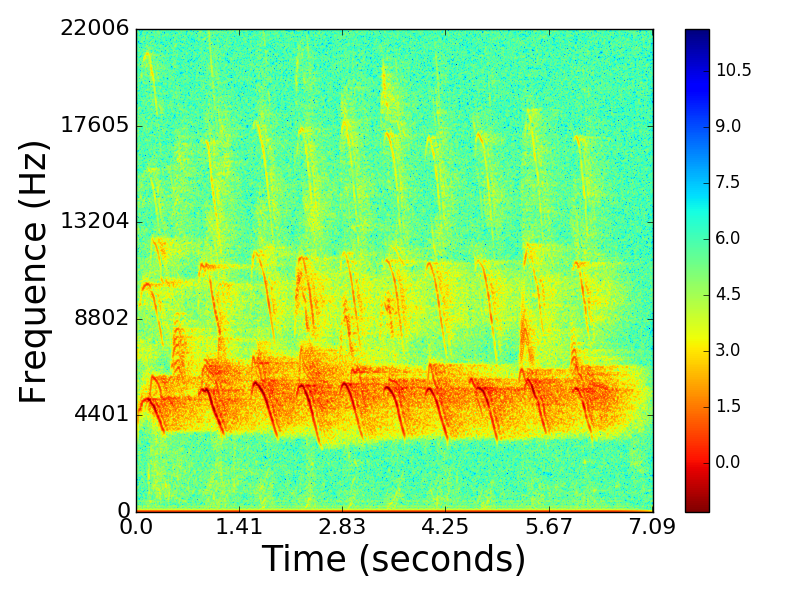
\includegraphics[height=4cm, width=0.55\textwidth]{examples/data/DOLPHINS_1024.png}
\end{frame}








% -----------------------------------------
\begin{frame}[fragile]
\frametitle{Rules}
\begin{center}

      \begin{minipage}{11cm}
        \begin{block}{}
            \begin{lstlisting}[basicstyle=\large]
rule spectrogram:
    input:  "DOLPHINS.wav"
    output: "DOLPHINS.png"
    shell: "python spectrogram.py {input}"
        \end{lstlisting}
         \end{block}        
        \begin{block}{Snakefile}
      Save the rule in a file called \textbf{Snakefile}. 
      \end{block}
    \end{minipage}
 \end{center}
\end{frame}

% -------------------------------

\begin{frame}[fragile]
\frametitle{Execution}
\begin{columns}[T]
\begin{column}[T]{5.3cm}
  \begin{block}{}
            \begin{lstlisting}
rule spectrogram:
    input:  "DOLPHINS.wav"
    output: "DOLPHINS.png"
    shell: "python spectrogram.py {input}"
    \end{lstlisting}
  \end{block}
\end{column}

\begin{column}{5.8cm}
      \begin{block}{Execution (in a shell)}
	  \begin{lstlisting}[basicstyle=\large]
	  snakemake
	  snakemake -s Snakefile
	  \end{lstlisting}
      \end{block}
      \end{column}
 \end{columns}
    \begin{block}{Stdout}
    \centering
    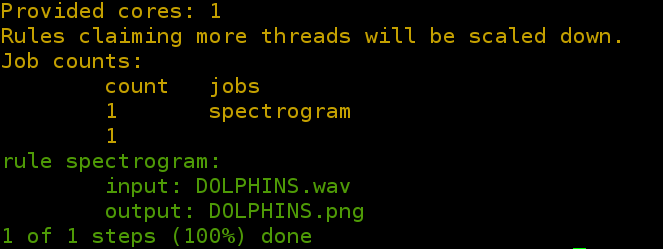
\includegraphics[scale=0.3]{examples/snakefile1/screen1.png}
    \end{block}     
\end{frame}

\begin{frame}    
    \centering
    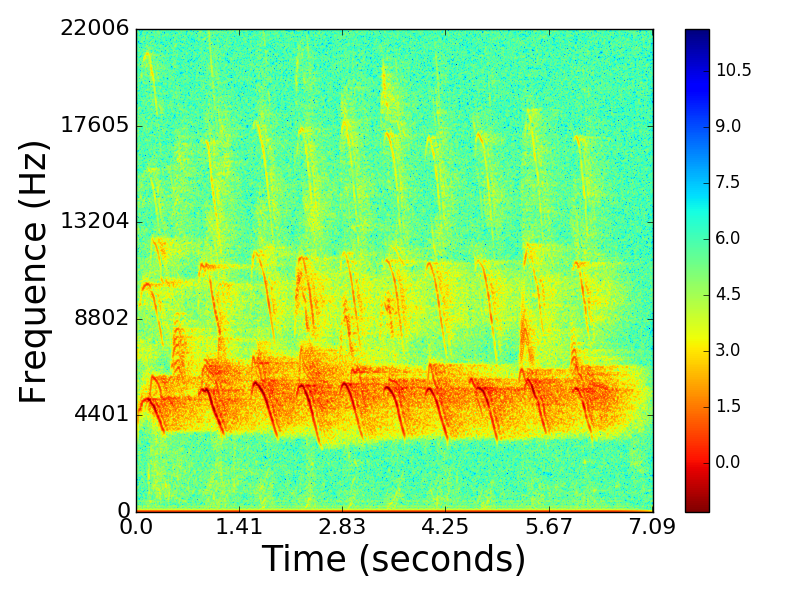
\includegraphics[height=8cm, width=1.1\textwidth]{examples/data/DOLPHINS_1024.png}
\end{frame}


% -----------------------------------------------------------
                
\begin{frame}[fragile]
\frametitle{Wildcards}
\small
\only<1>{
\begin{block}{}
Wildcards can be used to generalize a rule.
\end{block}
}
\only<2>{
\begin{block}{}
Snakemake automatically resolved multiple named wildcards.
You still need to set the final targets.
\end{block}
}
\only<3>{
\begin{block}{}
If the rule's output matches a 
requested file, the substrings  matched by the wildcards are 
propagated to the input files and to the variable wildcards
\end{block}
}
\begin{center}
    \begin{minipage}{11cm}
        \begin{onlyenv}<1>            
            \begin{block}{Wildcards}
                \begin{lstlisting}[basicstyle=\large]
            
            
       
  
rule sort:
    input:  "{dataset}.wav"
    output: "{dataset}.png"
    shell: "python spectrogram.py {input}"  
                  \end{lstlisting}    
               \end{block}

            \end{onlyenv}        
    
    \begin{onlyenv}<2>   
        \begin{block}{Wildcards}
            \begin{lstlisting}[basicstyle=\large]            
            
rule all:
  input: ["DOLPHINS.png", "WHALES.png"]
  
rule sort:
    input:  "{dataset}.wav"
    output: "{dataset}.png"
    shell: "python spectrogram.py {input}"  

    \end{lstlisting}    
        \end{block}
             \end{onlyenv}

         
    \begin{onlyenv}<3>  
        \begin{block}{Wildcards + expands + variables}
            \begin{lstlisting}[basicstyle=\large] 
samples = ['DOLPHINS', 'WHALES']            
rule all:
  input: expand("{name}.png", name=samples)

rule sort:
    input:  "{dataset}.wav"
    output: "{dataset}.png"
    shell: "python spectrogram.py {input}"
           \end{lstlisting}     
  \end{block}
     \end{onlyenv}        
    \end{minipage}
 \end{center}
 
\end{frame}
        
% ---------------------------
      
\begin{frame}[fragile]
\frametitle{Several wildcards}
   \begin{minipage}{12cm}
  \begin{block}{}
            \begin{lstlisting}[basicstyle=\large]
samples = ["DOLPHINS", "WHALES"]
windows = [512, 1024, 2048, 4096]

rule all:
    input: expand("{name}_{ws}.png", 
                          name=samples, 
                          ws=windows)

rule spectrogram:
    input: "{dataset}.wav"
    output: "{dataset}_{window}.png"
    shell: 
      "python spec.py {input} {wildcards.window}"
            \end{lstlisting}
  \end{block}
\end{minipage}
\end{frame}
  
        

\begin{frame}[fragile]
    \frametitle{Running snakemake}
      If all your files are in the current directory:
            \begin{lstlisting}[language=bash]
            snakemake
            \end{lstlisting}
      If you want to run on 4 cores:
            
            \begin{lstlisting}[language=bash]
            snakemake --cores 4
            \end{lstlisting}
      Dry run      
            \begin{lstlisting}[language=bash]            
            snakemake -n
            \end{lstlisting}
      Dry run and print shell commands
            
	  \begin{lstlisting}[language=bash]            
            snakemake -n -p
          \end{lstlisting}  
                
\end{frame}

% ----------------------------------------------

\begin{frame}[fragile]
    \frametitle{Config file}
     We can use a configuration file for parameters. Format are either JSON or YAML
    The community seems to prefer YAML.
    
    \begin{block}{config.yaml}
        \begin{lstlisting}
samples: [DOLPHINS, WHALES]
windows: [512,1024,2048,4096]
        \end{lstlisting}
    \end{block}
    \begin{block}{Snakefile}
    \begin{lstlisting}
configfile: "config.yaml"

rule all:
    input: expand("{name}_{ws}.png", 
                          name=config['samples'], 
                          ws=config['windows'])

rule spectrogram:
    input: "{dataset}.wav"
    output: "{dataset}_{window}.png"
    
    shell: 
      "python spec.py {input} {wildcards.window}"
    \end{lstlisting}
    \end{block}
\end{frame}


\begin{frame}[fragile]
 \frametitle{Add a rule without input/output}
 
 We could add a cleanup rule:
 
 \begin{block}{}
 \begin{lstlisting}
  rule clean:
      shell: "rm -f DOL*png WHALE*png"
    \end{lstlisting}
 \end{block}

 Since the rule does not produce any outputs and does not depend on other rules, 
 it is not part of the workflow: the rule must be called explicitly:
 
 
 \begin{block}{}
 \begin{lstlisting}[language=bash]
 snakemake clean
 \end{lstlisting}
 \end{block}
 
 \begin{alertblock}{dependencies}
  If not target is specified, snakemake tries to apply the first rule in the workflow
  Do not put the clean rule at the beginning !
 \end{alertblock} 
\end{frame}

% -------------------------------------------------------------


\begin{frame}[fragile]
 \frametitle{Handle logs}    
    \begin{block}{}
    \begin{lstlisting}[basicstyle=\small]
configfile: "config.yaml"

rule all:
    input: expand("data/{name}_{ws}.png", 
                          name=config['samples'], 
                          ws=config['windows'])

rule spectrogram:
    input: "data/{dataset}.wav"
    output: "data/{dataset}_{window}.png"
    log: "logs/{dataset}_{window}.log"
    shell: 
      "python spec.py {input} {wildcards.window} > {log}"
    \end{lstlisting}
    \end{block} 
\end{frame}

% -------------------------------------------------------------------

\begin{frame}[fragile]
 \frametitle{The \textbf{param} and \textbf{run} keywords}
   \begin{block}{}
    \begin{lstlisting}[basicstyle=\small]
rule all:
    input: 
      expected_output_list,
      "server.ready"

rule server:
  output: touch("server.ready")
  params: 
    port=config['port']
  run:  # Some python code
    from easydev import browse
    browse("http://127.0.0.1:%s" % params['port'])

rule spectrogram:
    ....
    \end{lstlisting}
    \end{block} 
\end{frame}

% ---------------------------------------------

\begin{frame}[fragile]
    \frametitle{onsuccess section}    
    If the workflow succeeds, the onsuccess section is ran if provided
    (same for onerror section).

    \begin{block}{}
    \begin{lstlisting}[basicstyle=\large]
onsuccess:
  from myapp import SpecExample
  app = SpecExample(samples, window, "data")
  app.launch(port=config['port'])
    \end{lstlisting}
    \end{block}
    
    You also have a \textbf{onerror} and \textbf{onstart} sections if needed.
\end{frame}

% --------------------------------

\begin{frame}[fragile]
\frametitle{demo}
Get materials from  

\url{https://github.com/sequana/sequana_presentations/2016/snakemake_IPday_dec/examples}
\begin{block}{}
    \begin{lstlisting}[basicstyle=\large]
snakemake -s spectrogram.rules \
          --configfile config.yaml \
          --cores 2  \
          --forceall
\end{lstlisting}
\end{block}
\end{frame}

% ----------------------------------------------------------------

\begin{frame}
\begin{block}{}
 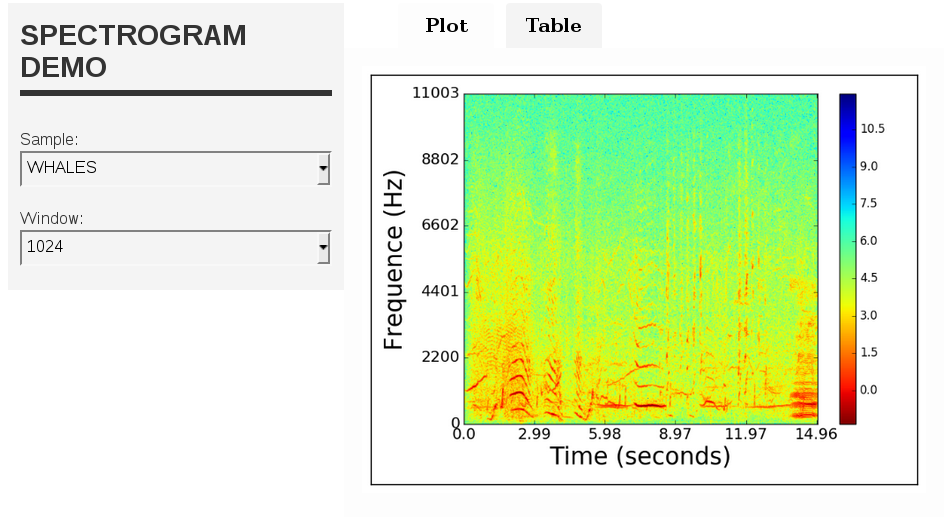
\includegraphics[scale=0.32]{examples/results.png}
\end{block}
\end{frame}


% ------------------------------------------------------------


\section{Advanced topics}
\begin{frame}[plain]
 \centering
 \begin{Huge}
Advanced topics 
\\
\large{alternative title: cheeries on the cake}
\end{Huge}
\end{frame}

% -----------------------------------------------------------------

\begin{frame}
\frametitle{Job execution \tiny{(source: J. Koster talk)}}
 A job is executed if
 \begin{itemize}
 \item  output file target does not exist
 \item  output file needed by another executed job and does not exist
 \item  input file newer than output file
 \item  input file will be updated by other job
 \item  execution is enforced
\end{itemize}
determined via breadth-first-search on DAG of jobs 
\end{frame}


% ---------------------------------------------------------------------



\begin{frame}[fragile]
\frametitle{threading}
Disjoint paths in the DAG of jobs can be executed in parallel using -\--cores 
argument:
\begin{lstlisting}
     snakemake --cores 8
\end{lstlisting}
We can be more specific inside the rules:
\begin{lstlisting}
        rule bwa_mapping:
            input: test.fastq
            output: test.bam
            threads: 4 
            shell: bwa mem -t {threads} {input} > {output}
\end{lstlisting}
 And use the same command:
 \begin{lstlisting}
    snakemake --cores 8
 \end{lstlisting}
 but here only two jobs are executed at the same time
\end{frame}
 
 % ----------------------------------------------
 
\begin{frame}[fragile]
\frametitle{resources (memory)}
We can be specific about memory used by a job with the resources keyword:
\begin{lstlisting}
        rule bwa_mapping:
            input: test.fastq
            output: test.bam
            threads: 4 
            resources: mem_mb=1000
            shell: bwa mem -t {threads} {input} > {output}
 \end{lstlisting}
  
and use the resources parameter when calling Snakemake:  
  \begin{lstlisting}
  # execute with only 8 cores and 1Gb memory
  
  snakemake --cores 8 --resources mem_mb=1000
  \end{lstlisting}   
  
  so here only one job at a time is executed
  
\end{frame}
 
% -----------------------------



\begin{frame}[fragile]
\frametitle{Cluster execution}

No intrusive code. It just worked on SGE and then on a SLURM cluster 
without changing a single line of code !

\begin{lstlisting}
# execute the workflow on cluster with qsub submission command
# (and up to 100 parallel jobs)
snakemake --cluster qsub --jobs 100

# tell the cluster system about the used threads
snakemake --cluster "qsub -pe threaded {threads}" --jobs 100

# execute the workflow with DRMAA
snakemake --drmaa --jobs 100

# execute the workflow on cluster with sbatch (SLURM)
snakemake --cluster "sbatch --qos fast" --jobs 100

\end{lstlisting}
\end{frame}


\begin{frame}
 \frametitle{Errors}
 
 If an error occurs after hours of computation, fix the error in your code or missing files, 
 and run snakemake again. Finished jobs won't be re-run. 
 
\end{frame}


\begin{frame}
\frametitle{other features}

\begin{itemize}
\item handles temporary and protected files
\item run until a given rule
\item run from a given rule
\item stats about run time
\item benchmark: run several times the rules
\item any external scripts can be used (R, python, etc)
\item remote files (http, ftp, google could, amazon, dropbox)
\item rules may have priorities
\item cluster time and memory can be fully customized
\item modular: can include rules, or sub workflow
\end{itemize}

\end{frame}

 
 
\section{Conclusions and discussions}
\begin{frame}[plain]
 \centering
 \begin{Huge}
Conclusions and discussions
\end{Huge}
\end{frame}

 
\begin{frame}
 \frametitle{Conclusions}
 
 \begin{block}{Mature}
  Snakemake is a mature tool ready for production. 
\end{block}

\begin{block}{batteries included}
 To cite just one great feature: free parallelization on a cluster.
\end{block}

\begin{block}{Nice Syntax}
The syntax is in Python, the library is in Python. Nevertheless, 
only a minimalist knowledge is required to get started since 
nice functions are already provided (e.g. expand).
\end{block}

\begin{block}{Large community}
Large snakemake community. See also the conda/bioconda community.
\end{block}

\end{frame}

 
\begin{frame}
\frametitle{Discussions}

\begin{block}{}
Snakemake is great so what's wrong ? 
\end{block}

\begin{block}{Not much but here are some food for thoughts}
\begin{itemize}
 \item Snakefile uses Python syntax but Snakefile are not Python module
 \item Errors are sometimes too cryptic and definitely not useful for end-users
 \item Despite lots of sanity checks, if you are not careful you may end up 
       in an infinite loop or delete the content of a file. So do lots of testing
       and save your data files before production. And just avoid symbolic links
       same input/output filenames.
 \item The rule syntax is great but developpers makes different choices on 
  how they use them. So despite a great idea of sharing tools, you end up 
  with many different pipelines and rules that does the same thing...
\end{itemize}
%  2 rule all:
%  3     input: "test.txt"
%  4 
%  5 rule A:
%  6     input: "test.txt"
%  7     output: touch("test.txt")
%  8     message: "okido"

\end{block}



Python is great but at the end it is not python ! rules are not 
Rules are supposed to be shared yet everybody is redoing its own pipeline and rules. It means it is not re-usable easily ! Need more abstraction
Syntax is makefile syntax so it must be a dag. No loop
\end{frame}

% -----------------------------------------------

\begin{frame}
    \frametitle{References}
    \begin{itemize}
        \item Great documentation for developers on Snakemake web site:
        \begin{itemize}
	    \item {\tiny https://bitbucket.org/snakemake/snakemake/wiki/Documentation}
            \item {\tiny https://bitbucket.org/snakemake/snakemake/wiki/Home}
        \end{itemize}        
        \item Useful information:
        \begin{itemize}
            \item {\tiny http://slides.com/johanneskoester/deck-1}
            \item {\tiny http://snakemake.bitbucket.org/snakemake-tutorial.html}
            \item {\tiny http://slowkow.com/notes/snakemake-tutorial/}
            \item {\tiny http://watson.nci.nih.gov/{\textasciitilde{}}sdavis/blog/flexible\_bioinformatics\_pipelines\_with\_snakemake/}
        \end{itemize}
        \item This talk and materials
        \\
        {\normalsize All snakefiles and data files to play 
	  around and available on}
        {\tiny https://github.com/sequana/presentations/2016/snakemake}       
        
    \end{itemize}
    
    \begin{block}{Snakemake Citations}
    {\tiny 
    K\"oster J., Rahmann S. 
    Snakemake -- a scalable bioinformatics workflow engine.    \\
    Bioinformatics application note  Vol 28 (19) 2012 }
    \end{block}
  
        
\end{frame}




% -----------------------------------------------

\begin{frame}[fragile]
\frametitle{Acknowlegments}
\centering
\pause
\begin{lstlisting}
HELPERS = [
    "Dimitri Desvillechabrol",
    "Rachel Legendre",
    "Christiane Bouchier",
    "The bioinformatics and biostatistics Hub (IP)"]

rule thank:
    input: expand("{helpers}", helpers=HELPERS)

rule you:
    output: temp(touch("{to}"))
\end{lstlisting}
\pause
\begin{block}{}
\begin{lstlisting}
 snakemake -s thanks.rules --dag | dot -Tpng >  thanks.png
\end{lstlisting}
\end{block}

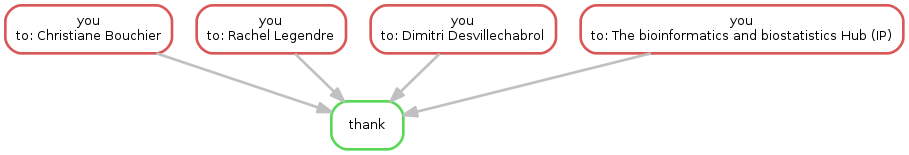
\includegraphics[scale=0.3]{examples/thanks.png}
\end{frame}

% --------------------------------------------------------

\begin{frame}[plain]
 \centering
 \begin{Huge}
  Questions 
 \end{Huge}
\end{frame}

 

% ---------------------------------------------

\begin{frame}[fragile]
    \frametitle{What happens when the snakemake is interrupted}
    \begin{itemize}
        \item If you stop your snakemake (i.e. ctrl+c):
        \begin{lstlisting}[language={}]
Terminating processes on user request.
Will exit after finishing currently running jobs.
Removing output files of failed job samtools since they might be corrupted:
reference.fa.fai
        \end{lstlisting}
        \item On the cluster, the current job is not kill
        \item If you close your shell (Crash simulation):
        \begin{lstlisting}[language={}]
IncompleteFilesException:
The files below seem to be incomplete. If you are sure that certain files are 
not incomplete, mark them as complete with

    snakemake --cleanup-metadata <filenames>

To re-generate the files rerun your command with the --rerun-incomplete flag.
Incomplete files:
ERR036019_unsort.bam
        \end{lstlisting}
        \item We can rerun the snakemake with \lstinline[basicstyle=\small\ttfamily]{--rerun-incomplete}.
    \end{itemize}
\end{frame}

\end{document}
